\section{Datenbank}

\subsection{Aufbau der SQLITE Datenbank}

Die Datenbank der App hat folgende Tabellen und Felder.

\begin{table} [htbp]
	\begin{center}
		\begin{tabular}{|l|l|l|}
			\rowcolor{black} {\color{white}\textbf{}} & {\color{white}\textbf{Typ}} & {\color{white}\textbf{Key}} \\
			\textbf{Items} & &  \\ \hline
			\rowcolor{DarkSeaGreen} ITEM\_ID & Integer & Ja \\ \hline
			EAN & Integer & \\ \hline
			\rowcolor{DarkSeaGreen} TITLE & String & \\ \hline	
			RATING & Integer & \\ \hline
			\rowcolor{DarkSeaGreen} MEDIA\_TYPE & String & \\ \hline
			GENRE\_ID & Integer & \\ \hline
			\rowcolor{DarkSeaGreen} LANGUAGE\_ID & Integer & \\ \hline
			LAUNCH & String \\ \hline
			\rowcolor{DarkSeaGreen} RENTAL & Integer & \\ \hline
			PUBLISHER\_ID & Integer & \\ \hline
			\rowcolor{DarkSeaGreen} AUTHOR\_ID & Integer & \\ \hline
			SYSTEM\_ID & Integer & \\ \hline
			\rowcolor{DarkSeaGreen} DVD & Integer & \\ \hline
			BLURAY & Integer & \\ \hline
			\rowcolor{DarkSeaGreen} STUDIO\_ID & Integer & \\ \hline
			DIRECTOR\_ID & Integer & \\ \hline
			\rowcolor{DarkSeaGreen} PARENTAL & Integer & \\ \hline
			REMARKS & String & \\ \hline
			\rowcolor{DarkSeaGreen} \textbf{History} & & \\ \hline
			HISTORY\_ID & Integer & Ja \\ \hline
			\rowcolor{DarkSeaGreen} ITEM\_ID & Integer & \\ \hline
			FRIEND\_ID & Integer & \\ \hline
			\rowcolor{DarkSeaGreen} START & String & \\ \hline
			BACK & String & \\ \hline
			\rowcolor{DarkSeaGreen} \textbf{Friends} & & \\ \hline
			FRIEND\_ID & Integer & Ja \\ \hline
			\rowcolor{DarkSeaGreen} FIRST\_NAME & String & \\ \hline
			LAST\_NAME & String & \\ \hline
			\rowcolor{DarkSeaGreen} \textbf{Authors} & & \\ \hline
			AUTHOR\_ID & Integer & Ja \\ \hline
			\rowcolor{DarkSeaGreen} AUTHOR & String & \\ \hline 
		\end{tabular}
		\caption{Datenbankfelder}
		\label{tab:Datenbankfelder}
	\end{center}
\end{table}

\newpage

\begin{landscape}
	\subsection{Übersicht Datenbank}
	\label{subsec:UebersichtDB}
	\begin{figure}[htbp]
		\centering
		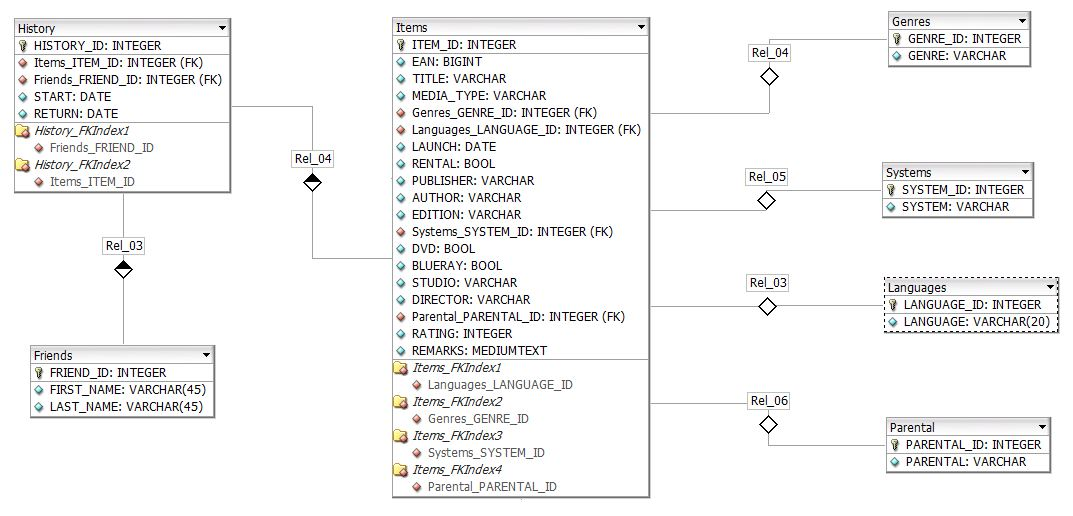
\includegraphics[scale=0.6]{pic/DbDesign}
		\caption{Überblick Datenbank}
	\end{figure}
\end{landscape}